\part{Constraints}
\begin{multicols}{2}
So far, the motion of particle was defined by forces:
\begin{itemize}
	\item Elastic springs,
	\item Damping,
	\item Gravity
\end{itemize}
motion is unrestricted using these techniques. Sometimes we want to restrict motion:
\begin{itemize}
	\item Bead a wire (constant length),
	\item Incompressible deformations (constant volume).
\end{itemize}
 \emph{Constraints} can be use to strictly \emph{enforce conditions} (unlike elastic forces) or to \emph{derive general forces} (unlike springs).

\begin{definition}{Constraint}
	A constraint $C(x_1, x_2, \ldots, x_n)$ is 
	\begin{itemize}
		\item A scalar-valued function of one or several arguments
		\item An implicit expression for a relation that must hold between its arguments.
	\end{itemize}

	\textbf{Convention}: A constraint is satisfied if $\mathbf{C=0}$.
\end{definition}
Examples of $n$-ary constraints:
\begin{itemize}
	\item Constant position $C_1(x_1)$
	\item Constant length $C_2(x_1, x_2)$
	\item Constant area $C_3(x_1, x_2, x_3)$
	\item Constant volume $C_4(x_1, x_2, x_3, x_4)$
\end{itemize}
\begin{figure}[H]
	\centering
	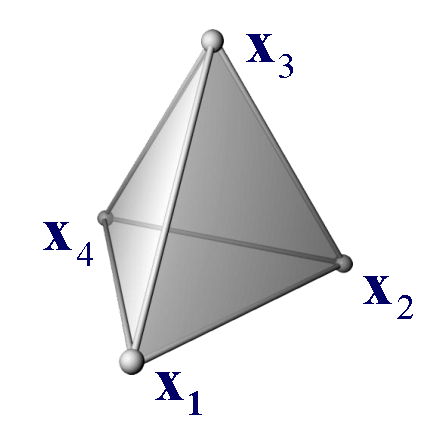
\includegraphics[width=0.25\textwidth]{img/02_tetra}
\end{figure}

\section{Soft constraints and the Penalty Method}
How can we enforce constraints? \\

Define potential energy for constraint:
\begin{align*}
	E_c(x_1, x_2, \ldots, x_n) = {1 \over 2} kC(x_1, x_2, \ldots, x_n)^2,
\end{align*}
where $k$ is a \emph{stiffness} coefficient.
\begin{align*}
	E_c &= 0 &\text{constraint is met},\\
	E_c &> 0 &\text{otherwise}.
\end{align*}
The \emph{constraint force} is a \emph{negative gradient} of potential energy:
\begin{align*}
	F_j = - {\delta E_c \over \delta x_j} = - kC(x_1, \ldots x_n){\delta C(x_1,\ldots, x_n) \over \delta x_j}
\end{align*}
The \emph{penalty force} pulls the system towards $\mathbf{C=0}$.

\paragraph{Distance Preservation} Preserve distance between two points:
\begin{align*}
	C(x_0, x_1) &= \norm{x_1-x_0}-L\\
	F_1^C(x_0, x_1) &= -kC(x_0, x_1){\delta C(x_0, x_1) \over \delta x_1}\\
		&= \underbrace{-k(\norm{x_1-x_0}-L){x_1-x_0 \over \norm{x_1-x_0}}}_\textbf{Spring Force}
\end{align*}

\paragraph{Simulation with Penalty Forces} Simulate $x_0$ and $x_1$ using Newton's law. Enforce distance constraint with penalty forces:
\begin{align*}
 F_i^C(x_0, x_1) &= -kC(x_0, x_1){\delta C(x_0, x_1) \over \delta x_i}
\end{align*}
Step forward in time (explicit Euler):
\begin{align*}
	v_{n+1} = v_n + h {1 \over M}\left( F^C (x) + F^{ext} \right).
\end{align*}
\end{multicols}

\subsubsection{Recipes for constraint forces}
\begin{description}
	\item[Area of a triangle] $(x_0, x_1, x_2)$:
		\begin{align*}
			C(x_0, x_1, x_2) = {1\over 2} \norm{(x_1-x_0) \times (x_2-x_0)}-A
		\end{align*}
	\item[Volume $\mathbf V$ of a tetrahedron] $(x_0, x_1, x_2, x_3)$:
		\begin{align*}
			C(x_0, x_1, x_2, x_3) = {1\over 6} (x_1-x_0) \cdot \left[ (x_2-x_0) \times (x_3-x_0) \right]-V
		\end{align*}
\end{description}

\subsection{Summary Soft Constraints}
Constraint forces are:
\begin{itemize}
	\item A powerful mechanism to enforce various conditions,
	\item Generic: Express condition, forces from a standard scheme,
	\item $n$-ary forces as opposed to binary strings.
\end{itemize}

\emph{However}, constraints can be:
\begin{itemize}
	\item Computationally expensive (especially with implicit integration),
	\item Redundant or conflicting,
	\item Penalty forces \emph{model \textbf{soft} constraints} and are \emph{not sufficient} for strict enforcement (\emph{\textbf{hard} constraints}).
\end{itemize}

\begin{multicols}{2}
\section{Hard Constraints}
How can we model a hard constraint? Consider a 2D particle constrained to move on a unit circle.
\begin{figure}[H]
\centering
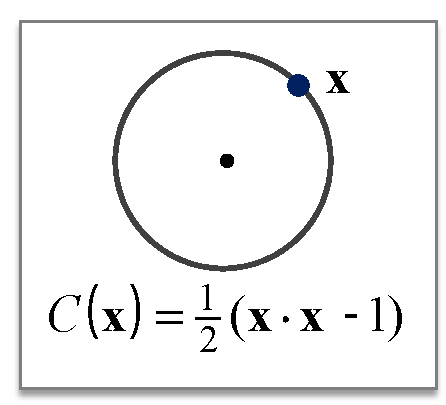
\includegraphics[width=0.40\textwidth]{img/02_hard_constraints_circle}
\end{figure}
First we define \emph{legal} kinematics:
\begin{align*}
	\textbf{Position: }&C(x) = 0\\
	\textbf{Velocity: }&\dot C(x) = 0\\
	\textbf{Acceleration: }&\ddot C(x) = 0
\end{align*}
\textbf{Idea:} Start with a legal position and velocity and ensure that acceleration remains legal (constraint forces).
\begin{align*}
	&\begin{cases}
	\underbrace{\ddot C(x) = \ddot x \cdot x + \dot x \cdot \dot x = 0}_\text{Legal acceleration}\\
	\underbrace{ \ddot x = {F + F^C \over m} }_\text{Newton's Law}
	\end{cases}\\
	 &\text{combine:}\\
	&F^C \cdot x = -F\cdot x - m\dot x \cdot \dot x
\end{align*}
Require constraint force to act only in gradient direction:
\begin{align*}
	F^C = \lambda {\delta C \over \delta x} = \lambda x.
\end{align*}
Insert into combined formula:
\begin{align*}
	\lambda = - {F\cdot x + m \dot x \cdot \dot x \over x \cdot x},
\end{align*}
which gives us an \emph{hard constraint force}.

\paragraph{Simulation with Hard Constraints} Use hard constraints with an explicit function (since implicit integration is (much) more complicated):
\begin{enumerate}
	\item Solve (LES) for constraint force magnitudes $\lambda_n$.
	\item Compute constraint forces:
		\begin{align*}
			F_n^C &= {\delta C(x_n)^t \over \delta x}\lambda_n
		\end{align*}
	\item Step forward in time 
		\begin{align*}
			v_{n+1} = v_n + {h\over M} \left(F_n^C + F^{ext}\right)
		\end{align*}
\end{enumerate}

\subsection{Summary Hard Constraints}
Hard constraint forces
\begin{itemize}
	\item add just enough force to maintain constraint (exactly),
	\item require no high stiffness (numerically pleasing).
\end{itemize}
However
\begin{itemize}
	\item \emph{Constraints drift} (error in ODE solve), needs correction
	\item General formulation is more involved (many constraints)
	\item Requires the solution of systems of equations
\end{itemize}





\end{multicols}


